%----------------------------------------------------------------------------------------
%
% CHAPTER TWO
%----------------------------------------------------------------------------------------
\chapter{THEORETICAL FOUNDATIONS}
\label{ch:ch2}
\textcolor{red}{ In recent years, 2D materials have emerged as a fascinating class of materials with unique properties and promising applications in various fields ranging from electronics and photonics to energy and biotechnology. These materials, which exhibit extraordinary properties due to their ultrathin nature, are reshaping the landscape of materials science and engineering. Among the diverse array of 2D materials, graphene, transition metal dichalcogenides (TMDs), hexagonal boron nitride (\gls{h-BN}), and other emerging candidates stand out for their exceptional characteristics and potential applications. We introduce 2D materials with a tyical hexagonal lattice nanostructure and their crystallography properties in this chapter. We then introduce the tight-binding approach, which is basic for understanding the electronic properties of materials, with a particular focus on the nearest neighbor tight-binding model. We also discuss the electron dynamics in 2D materials, including the time-dependent Schrödinger equation and quantum master equation which are fundamental for studying the nonlinear optical response in this thesis. We introduce several typical 2d materials:}

\textcolor{red}{	Graphene: a single layer of carbon atoms arranged in a honeycomb lattice, is the archetype of 2D materials. Graphene exhibits mechanical strength, electrical conductivity, and thermal conductivity. Its unique electronic band structure and optical properties make it a versatile material for various applications in electronics, such as high-speed transistors and flexible displays, as well as in energy storage, sensors, and biomedical devices.}

\textcolor{red}{Hexagonal Boron Nitride (\gls{h-BN}):  a structural analog of graphene, consists of alternating boron and nitrogen atoms arranged in a hexagonal lattice. \gls{h-BN} exhibits excellent thermal and chemical stability, as well as a large bandgap, making it an insulating material. Its flat and atomically smooth surface makes it an ideal substrate for 2D materials and a protective coating in electronic devices. It is widely used as a dielectric material in transistors, tunneling barriers in spintronics.}

\textcolor{red}{Transition Metal Dichalcogenides (TMDs): a class of 2D materials composed of transition metal atoms sandwiched between two layers of chalcogen atoms (e.g., sulfur, selenium, or tellurium). TMDs exhibit intriguing electronic, optical, and mechanical properties, which can be tuned by varying the composition and layer thickness. They often possess a direct bandgap, making them suitable for optoelectronic applications. They are used in field-effect transistors, photodetectors, light-emitting diodes (LEDs), and other optoelectronic devices. They also hold promise in catalysis, sensing, and flexible electronics.}

\textcolor{red}{Other Emerging 2D Materials like Black Phosphorus: a layered semiconductor, offers tunable bandgap and high carrier mobility, making it suitable for electronic and optoelectronic applications. MXenes are a family of 2D transition metal carbides, nitrides, and carbonitrides with metallic conductivity and excellent mechanical properties, holding promise in energy storage, catalysis, and electromagnetic shielding. Perovskite Nanosheets: Perovskite nanosheets exhibit remarkable photophysical properties and are being explored for applications in solar cells, photodetectors, and light-emitting devices.}

\textcolor{red}{In summary, 2D materials, including graphene, TMDs, \gls{h-BN}, and other emerging candidates, offer a rich platform for exploring novel physical phenomena and developing advanced technologies with unprecedented performance and functionality. Their diverse properties and potential applications make them a vibrant area of research in materials science and engineering. The inclusion of artificial 2D materials based on moiré superlattices underscores the dynamic nature of this field and the potential for groundbreaking discoveries \cite{kennes2021moire}.}
%%%%%%%%%%%%%%%%%%%%%%%%%%%%%%%%%%%%%%%%%%%%%%%%%%%%%%%%%%%%%%%%%%%%%%%%%%%%%%%%%%%
\section{Crystallography Properties}
%%%%%%%%%%%%%%%%%%%%%%%%%%%%%%%%%%%%%%%%%%%%%%%%%%%%%%%%%%%%%%%%%%%%%%%%%%%%%%%%%%%
\textcolor{red}{Hexagonal lattice nanostructures are fundamental building blocks in the realm of 2D materials, encompassing a diverse range of materials with hexagonal symmetry. From natural materials like graphene and \gls{h-BN} to artificial structures based on moiré physics \cite{kennes2021moire}, the crystallographic properties of hexagonal lattices underpin the rich and varied behavior observed in 2D materials, offering ample opportunities for scientific exploration and technological innovation.}
As a fundamental Bravais lattice, it manifests as a distinctive geometric arrangement prevalent across a spectrum of materials, owing to its highly efficient packing characteristics. This lattice's spatial configuration profoundly influences the mechanical, electrical, and thermal properties of materials. Understanding lattice structures is crucial for deciphering material behavior across diverse conditions, spanning from semimetals to topological insulators. This significance is particularly noteworthy in the realm of two-dimensional materials. We have selected graphene, exemplifying a semimetal, and hexagonal boron nitride (h-BN), recognized as an insulator, for our discussion on nonlinear optical response on 2d materials.\\
\begin{figure}[htpb]
	\centering
	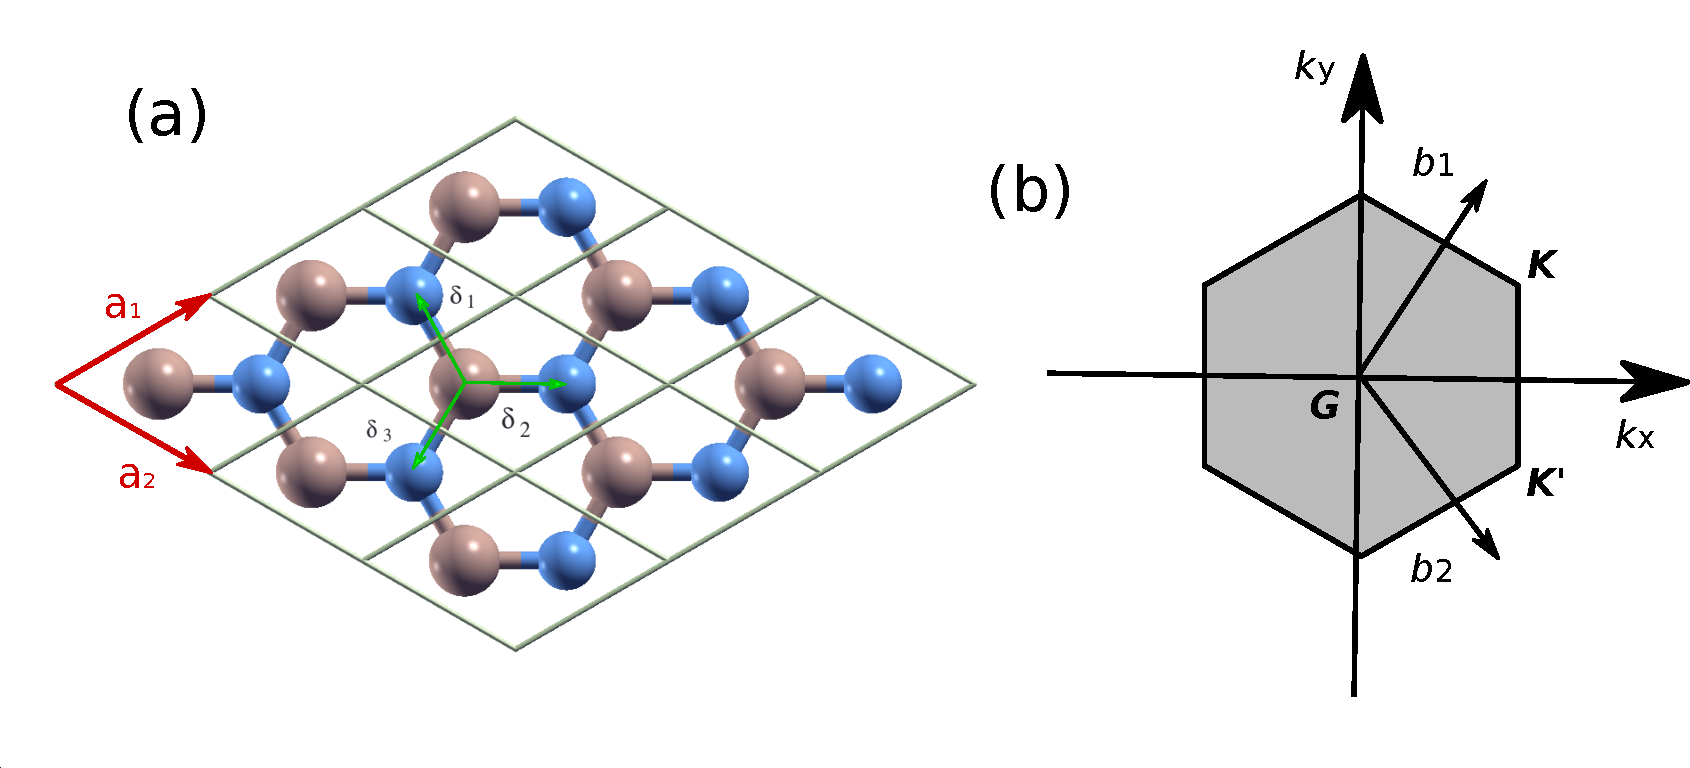
\includegraphics[width=0.96\textwidth]{pic/lattice.pdf}
	\caption[Lab coordinate system]{(a) Hexagonal lattice,the two triangular sublattices are shown
		in two different colors. (b) Brillouin zone in momentum space.}
	\label{fig: lattice}
\end{figure}
Graphene's lattice structure is hexagonal lattice nanostructure for carbon allotrope, showed in Figure \ref{fig: lattice} (a). Carbon atoms
lie in a single layer, forming an exceptional two-dimensional material. The unique
atomic-scale hexagonal lattice structure involves each carbon atom intricately bonding through
$\sigma$-bonds with its three nearest neighbors and a delocalized $\pi$-bond. This precise
arrangement plays a important role in the formation of Dirac cone, making monolayer graphene an outstanding conductor of electricity, and
finding applications in electronic devices, sensors, and various fields~\cite{sarma2011electronic}.

Similar to graphene, \gls{h-BN} also features a hexagonal lattice structure, but with alternating boron and nitrogen atoms forming the hexagons, making it a wide-gap insulator due to inversion symmetry breaking, which is used as a dielectric material in electronics, a substrate for graphene-based devices, and as a solid lubricant.
% begin{figure}[tb] % t = top, b = bottom, etc.
We define the basis of hexagonal lattice primitive vectors $E = (\vec{a}_{1}, \vec{a}_{2})$ as shown in Fig \ref{fig: lattice} (a):
$$
	\vec{a}_{1}=a\left(\begin{array}{l}
			\frac{\sqrt{3}}{2} \\
			\frac{1}{2}
		\end{array}\right),
	\vec{a}_{2}=a\left(\begin{array}{l}
			\frac{\sqrt{3}}{2} \\
			-\frac{1}{2}
		\end{array}\right)
$$
where $a$ is the lattice constant, for graphene $a= 1.42 \mathring{A}$ \cite{sarma2011electronic}, and for \gls{h-BN} $a= 2.5 \mathring{A}$ \cite{PhysRevB.81.155433}. Generate only $A$ sites while sites in $B$ sublattice are generated by $n_{1} \vec{a}_{1}+n_{2} \vec{a}_{2}+\vec{\delta},$ where $\vec{\delta}$ has to be chosen as one of the three nearest-neighbor vectors,
$$
	\begin{array}{c}
		\vec{\delta}_{1}=a\left(\begin{array}{l}
				                        -\frac{1}{2 \sqrt{3}} \\ \frac{1}{2}\end{array}\right),
		\vec{\delta}_{2}=a\left(\begin{array}{l}\frac{1}{\sqrt{3}}\\ 0 \end{array}\right),
		\vec{\delta}_{3}=a\left(\begin{array}{l} -\frac{1}{2 \sqrt{3}}\\ -\frac{1}{2}\end{array}\right)
	\end{array}
$$
The reciprocal basis $B=\left(b_{1}, b_{2}, b_{3}\right)$ is generated using the formula:
$$
	\overrightarrow{b_{k}}=\frac{2 \pi \cdot \overrightarrow{a_{i}} \times \overrightarrow{a_{j}}}{V}
$$
$i, j, k$ are circular permutations, $\mathrm{V}=\overrightarrow{a_{1}}\cdot (\overrightarrow{a_{2}}
	\times \overrightarrow{a_3})$, presents the mix product between the three vectors, i.e. the volume
of the unitary cell.  By assuming the lattice primitive vector in the vertical direction of the
two-dimensional material plane is infinit, $\overrightarrow{a_{3}}\to\infty$, we get the $2 \mathrm{D}$ reciprocal vectors as shown in Fig\ref{fig: lattice} (b):
$$
	\vec b_{1}=k_{D}\left(\begin{array}{l}
			\frac{1}{2} \\
			\frac{\sqrt{3}}{2}
		\end{array}\right),
	\vec b_{2}=k_{D}\left(\begin{array}{c}
			\frac{1}{2} \\
			-\frac{\sqrt{3}}{2}
		\end{array}\right)
$$
with $k_{D}=\frac{4 \pi}{\sqrt{3} a}$. The corresponding Brillouin zone is depicted together with the two high-symmetry points $\mathrm{K}$ and $\mathrm{K'}$ Fig ~\ref{fig: lattice} (b).
Two inequivalent corners of the Brillouin zone $K$ and $K^{\prime}$ can be chosen as follows:
$$
	K=k_{D}\left(\frac{1}{2}, \frac{1}{2 \sqrt{3}}\right), \quad K^{\prime}=k_{D}\left(\frac{1}{2},-\frac{1}{2 \sqrt{3}}\right)
$$

%%%%%%%%%%%%%%%%%%%%%%%%%%%%%%%%%%%%%%%%%%%%%%%%%%%%%%%%%%%%%%%%%%%%%%%%%%%%%%%%%%%
\section{Tight-binding Approach \label{sec:tightbinding}}
%%%%%%%%%%%%%%%%%%%%%%%%%%%%%%%%%%%%%%%%%%%%%%%%%%%%%%%%%%%%%%%%%%%%%%%%%%%%%%%%%%%

In this section, we delve into the fundamental principles of the tight-binding approach, with a particular focus on the nearest neighbor tight-binding model. This approach is essential for understanding the electronic properties of materials and is a crucial component of graphene's electronic structure analysis.
\textcolor{red}{In solid-state physics, the tight-binding model is a theoretical framework used to describe the electronic structure of crystalline materials. It treats each atomic orbital as a basis function and describes the electronic wavefunction as an expansion in terms of these basis functions. One common approach is to expand the wavefunction using Linear Combination of Atomic Orbitals (\gls{LCAO}). In this method, the wavefunction on position $r$ in the crystal lattice is expressed as a linear combination of atomic orbitals centered on individual atoms:}
\textcolor{red}{
	\begin{equation}
		\phi_{\beta}(\mathbf{r})=\sum_{\mathbf{R}_{\alpha}} b_{\beta}\left(\mathbf{R}_{\alpha}\right) \varphi_{\beta}\left(\mathbf{r}-\mathbf{R}_{\alpha}\right)
		\label{eq:lcao}
	\end{equation}
	Here, $b$ are coefficients for the linear combination, \beta$ is the general atomic orbitals index, $\varphi_{\beta}$ are the atomic orbitals which are eigenfunctions of the Hamiltonian $H_{\alpha}$ of a single isolated atom $\alpha$.
	The Bloch theorem states that the wave function in a crystal can change under translation only by a phase factor:
	\begin{equation}
		\phi\left(\mathbf{r}+\mathbf{R}_{\alpha}\right)=e^{i \mathbf{k} \cdot \mathbf{R}_{\alpha}} \psi(\mathbf{r})
		\label{eqn:bloch}
	\end{equation}
}
The foundation of the tight-binding approach is rooted in the Bloch theorem, which is satisfied by the tight-binding function by combining Eq.~(\ref{eq:lcao}) and Eq.~(\ref{eqn:Bloch}):
\begin{equation}
	\Phi_{\alpha,\beta}(\mathbf{r}, \mathbf{k})=\frac{1}{\sqrt{N}} \sum_{\mathbf{R}} e^{i \mathbf{k}
			\cdot \mathbf{R}} \phi_{\alpha,\beta}\left(\mathbf{r}-\mathbf{R}_{\alpha,\beta}\right), \alpha=A \text { or } B
	\label{eqn:Bloch}
\end{equation}
For simplicity, we only consider the contribution from the outermost valence band electron's
orbital and omit $\beta$ in the following discussion. $N$ represents the number of unit cells, and $\phi_{\alpha}(\mathbf{r} - \mathbf{R}_{\alpha})$ denotes the orbital function of an electron at cell $\mathbf{R}$ in sublattice $\alpha$.
In the context of a honeycomb lattice, we focus on the nearest neighbor approximation. This approximation asserts that an atom in sublattice A only interacts with its three closest neighbor atoms in sublattice B. This simplification is particularly useful for understanding the interactions between electrons bound to non-equivalent atoms.

The Hamiltonian for this nearest-neighbor interaction is expressed as:
\begin{equation}
	\hat{H}_{A B}=\frac{1}{N} \sum_{\mathbf{R}_{A}} \sum_{\mathbf{R}_{B}} e^{i \mathbf{k}\left(\mathbf{R}_{B}-\mathbf{R}_{A}\right)}\left\langle\phi_{A}\left(\mathbf{r}-\mathbf{R}_{\mathbf{A}}\right)|\hat H| \phi_{B}\left(\mathbf{r}-\mathbf{R}_{B}\right)\right\rangle
\end{equation}
Due to the translational invariance in a Bravais lattice, the summation over each atom in a sublattice occurs $N$ times, simplifying the expression to:
\begin{equation}
	\hat{H}_{A B}=\sum_{\mathbf{R}_{A}} e^{i \mathbf{k}\left(\mathbf{R}_{B}-\mathbf{R}_{A}\right)}\left\langle\phi_{A}\left(\mathbf{r}-\mathbf{R}_{\mathbf{A}}\right)|\hat{H}| \phi_{B}\left(\mathbf{r}-\mathbf{R}_{B}\right)\right\rangle
\end{equation}
We transform the Hamiltonian of real space into the momentum space representation, and then the
tight-binding Hamiltonian under the matrix representation is:
\begin{equation}
	\hat{H} =\left(\begin{array}{cc}
			\epsilon_{A}            & t_{0} f(\mathbf{k}) \\
			t_{0} f(\mathbf{k})^{*} & \epsilon_{B}
		\end{array}\right)
	\label{eqn: TBh}
\end{equation}

Here $\epsilon_{A}$ and $\epsilon_{B}$ are the on-site energies of electrons on the nearest neighbor atoms, $t_0$ presents the hopping parameter:
$$
	t_{0}=\left\langle\phi_{A}\left(\mathbf{r}-\mathbf{R}_{\mathbf{A}}\right)|\hat{H}| \phi_{B}\left(\mathbf{r}-\mathbf{R}_{A}-\vec{\delta}_{i}\right)\right\rangle \quad(i=1,2,3)
$$\\
For typical hexagonal lattice under our discussion, the three nearest neighbor hoping strength here are identical here due to the hexagonal lattice symmetry. For graphene, we set $\epsilon_{A}$ and $\epsilon_{B}$ to 0, and $t_0=2.8~eV$ in accordance with the previous work  \cite{sarma2011electronic}. For h-BN $\epsilon_{\mathrm{B}}$ and $\epsilon_{\mathrm{N}}$ denote the on-site energies for boron and nitrogen sites, respectively.
\begin{equation}
	\hat{H}(\mathbf{k})=\left(\begin{array}{cc}
			\epsilon_{\mathrm{B}}   & t_{0} f(\mathbf{k})   \\
			t_{0} f(\mathbf{k})^{*} & \epsilon_{\mathrm{N}}
		\end{array}\right),
	\label{eqn:hBNhamiltonian}
\end{equation}
We set $\epsilon_{\mathrm{B}}$ to $3.34$~eV and $\epsilon_{\mathrm{N}}$ to $-2.56~eV$ and $t_0$ to $2.6~eV$ computed with the first-principles calculations~\cite{PhysRevB.51.6868}, the band gap $E_{g}=\epsilon_{b}-\epsilon_{n}$ equals 5.9~eV.

The off-diagonal terms of the tight-binding Hamiltonian \ref{eqn: TBh}:
\begin{equation}
	\begin{aligned}
		f(\mathbf{k}) & =e^{i \mathbf{k} \vec{\delta}_{1}}+e^{i \mathbf{k} \vec{\delta}_{2}}+e^{i \mathbf{k} \vec{\delta}_{3}}  \\
		              & =e^{-\frac{i a k_{x}}{\sqrt{3}}}+2 e^{\frac{i a k_{x}}{2 \sqrt{3}}} \cos \left(\frac{a}{2} k_{y}\right)
	\end{aligned}
	\label{eqn:nearest_h}
\end{equation}
Solving the stationary Schrödinger equation using matrix diagonalization:
\begin{align}
	\hat{H}_{\mathbf{k}}|\phi_{b \mathbf{k}}\rangle = \epsilon_{b\mathbf{k}}|\phi_{b}\rangle,
	\label{eq:eqigenstates-h0}
\end{align}
we get the eigenenergy of Hamiltonian from \ref{eqn: TBh}, where $b$ is a band index, $|\phi_{b\mathbf{k}}\rangle$ is an eigenstate, and $\epsilon_{b\mathbf{k}}$ corresponds to the eigenenergy. As the Hamiltonian is a $2$-by-$2$ matrix in this work, the band index $b$ denotes either a conduction ($b=c$) or valence ($b=v$) state.

\begin{equation}
	\epsilon_{b\mathbf{k}}=E_{0} \pm \frac{1}{2} \sqrt{E_{g}^{2}+4t_{0}^{2}|f|^{2}}
	\label{eigenvalues}
\end{equation}
$E_{0}=\frac{\epsilon_{A}+\epsilon_{B}}{2}$ and $E_{g}=\epsilon_{b}-\epsilon_{n}$ is the energy gap. For graphene, $\epsilon_{A} = \epsilon_{B} =0$ the band gap equals 0.
Their corresponding eigenvectors are:
\begin{equation}
	|\phi_{b}\rangle  =\left(\begin{array}{cc}
			\frac{E_{g} \pm \sqrt{E_{g}^{2}+4t_{0}^{2}|f|^{2}}}{2t_{0} f^*} \\
			1
		\end{array}\right)
	\label{eqn:eigenvector}
\end{equation}
\color{red}

Tight-binding model is an approximation to the first principles models that can be drerived from ab-initio DFT calculations and used to improve computational effeciency through Wannierization. Wannierization facilitates the transformation of electronic wavefunctions from a basis of Bloch states to localized Wannier functions. Wannier functions provide a clearer physical interpretation of the electronic structure compared to Bloch states. Each Wannier function corresponds to an electron localized around a particular atomic site within the crystal lattice. This localization allows for a more intuitive understanding of electronic properties, such as onsite energy, bonding, hopping, and interactions, in terms of localized atomic-like orbitals. Wannierization can help educe the size of the Hilbert space, as the model focuses on the interactions between a limited number of localized orbitals rather than considering the entire Brillouin zone; provide a systematic method for constructing the tight-binding Hamiltonian; allow for the localization of these interaction terms around specific lattice sites, making the tight-binding model more physically intuitive and interpretable; moreover, enable the incorporation of additional physical effects, such as electron-electron interactions, spin-orbit coupling, and lattice distortions, into the tight-binding model.

In 2D materials, quantum effects become prominent due to the reduced dimensionality, leading to the emergence of novel electronic states and phenomena. Understanding how topological obstruction influences the electronic structure of 2D materials sheds light on the quantum behavior that governs their properties. For 2D systems, the quantity of topological index as a surface integral over the Brillouin Zone is defined as the Chern number:

\begin{align}
	W_{n}=\frac{1}{2 \pi} \iint_{B Z} d ^{2} \boldsymbol{k} \cdot \vec{\Omega}_{n}
\end{align}
Quantized Hall conductance $\sigma_{xy}$ can be calculated using the Chern number and the TKNN formula\cite{thouless1982quantized}:
\begin{align}
	\sigma_{xy}=\frac{e^2}{h}W_n
\end{align}
$\vec{\Omega}_n$ is the Berry curvature, which is defined as the curl(rotor) of the Berry connection or the
Berry vector potential $\mathcal{A}(\boldsymbol{k})=\left\langle n(\boldsymbol{k})\left|i \nabla_{\boldsymbol{k}}\right|n(\boldsymbol{k})\right\rangle
$\cite{berry1984quantal}. Barry phase $\gamma_n$ is expressed as a closed path $\mathcal{C}$ integral in the $\boldsymbol{k}$-space $\gamma_{n}=\oint_{\mathcal{C}} d \boldsymbol{k} \cdot \mathcal{A}_{n}(\boldsymbol{k})=\int_{\mathcal{S}} d \boldsymbol{k} \cdot \vec{\Omega}_{n}(\boldsymbol{k})$.
$n(\boldsymbol{k})$ denotes the $n^{th}$ eigenstate of the Bloch
Hamiltonian $H(\boldsymbol{k})$ for general systems. The Berry curvature $\vec{\Omega}_n$ is an intrinsic property of the
band structure because it only depends on the wave
function, which can be nonzero in crystals with broken time-reversal or inversion symmetry.\cite{xiao2010berry}
\begin{align}
	\vec{\Omega}_{n}(\boldsymbol{k})=\nabla_{\boldsymbol{k}} \times\mathcal{A}(\boldsymbol{k})
\end{align}

Using $\left\langle n|\partial H / \partial \boldsymbol{k}| n^{\prime}\right\rangle=\left\langle\partial n / \partial \boldsymbol{k} \mid n^{\prime}\right\rangle\left(E_{n}-E_{n^{\prime}}\right) \text { for } n^{\prime} \neq n$, the Berry curvature can be also written as a summation over the eigenstates:
\begin{align}
	\vec{\Omega}_{n}(\boldsymbol{k})=\operatorname{Im} \sum_{n^\prime \neq n} \frac{\left\langle n(\boldsymbol{k})\left|\nabla_{\boldsymbol{k}} H(\boldsymbol{k})\right| n^\prime(\boldsymbol{k})\right\rangle \times\left\langle n^\prime(\boldsymbol{k})\left|\nabla_{\boldsymbol{k}} H(\boldsymbol{k})\right| n(\boldsymbol{k})\right\rangle}{\left(E_{n^\prime}(\boldsymbol{k})-E_{n}(\boldsymbol{k})\right)^{2}}
\end{align}
which is useful to calculate the numerically the integral.\\

Hereafter, for two-band tight-binding model, $n(\boldsymbol{k})$ is the instantaneous eigenstates of the time-dependent Hamiltonian $H$ from Eq.~(\ref{eqn:vTD}) under the vector potential $\mathbf{A(t)}$.
$n(\boldsymbol{k})$ equals to $\phi_{v,\boldsymbol k+\mathbf A(t)}$ and $\phi_{c,\boldsymbol k+\mathbf A(t)}$ for the valence band and the conduction band.  One get the Berry curvature for conduction band of 2D-systems:
\begin{align}
	 & \vec{\Omega}_{c,k_xk_y}(\boldsymbol{k})=i  \frac{\left\langle \phi_c(\boldsymbol{k})\left|\partial H(\boldsymbol{k}) / \partial k_x\right| \phi_v(\boldsymbol{k})\right\rangle\left\langle \phi_v(\boldsymbol{k})\left|\partial H(\boldsymbol{k}) / \partial k_y\right| \phi_c(\boldsymbol{k})\right\rangle-(k_y \leftrightarrow k_x)}{\left(\epsilon_{c}(\boldsymbol{k})-\epsilon_{v}(\boldsymbol{k})\right)^{2}}
\end{align}
Normally, for monolayer graphene, inversion symmetry hodes $\Omega_n(\boldsymbol{-k})=\Omega_n(\boldsymbol{k})$. Also, the Berry curvature and momentum change sign under time-reversal, so that the Berry curvature at one momentum becomes opposite to the Berry curvature at opposite momentum $\Omega_n(\boldsymbol{-k})=-\Omega_n(\boldsymbol{k})$, so $\Omega_n(\boldsymbol{k})=0$ and $\sigma_{xy}=0$. \cite{xiao2010berry}. For non-centrosymmetric crystals, for instance monolayer hBN, inversion symmetry is broken but time reversal symmetry holds, we have $\Omega_n(\boldsymbol{k})\neq0$ and $\sigma_{xy}=0$. And if only time reversal symmetry broken but inversion symmetry holds, for instance magnetic materials, we have $\Omega_n(\boldsymbol{k})\neq0$ and $\sigma_{xy}\neq0$.

For graphene/hBN:
\begin{align}
	\frac{\partial H}{\partial \boldsymbol k}=
	\left(\begin{array}{cc}
			      0                                                                            & t_{0} \frac{\partial f(\boldsymbol{k}+\mathbf{A})}{\partial \boldsymbol k} \\
			      t_{0} \frac{\partial f^*(\boldsymbol{k}+\mathbf{A})}{\partial \boldsymbol k} & 0
		      \end{array}\right),
\end{align}


\begin{align}
	\frac{\partial f(\boldsymbol{k}+\mathbf{A})}{\partial \boldsymbol k}
	=i\vec {\delta}_1 e^{i\left (\boldsymbol k+\mathbf A \right ) \cdot \vec\delta_1}
	+i\vec{\delta}_2 e^{i\left (\boldsymbol k+\mathbf A \right ) \cdot \vec\delta_2}
	+i\vec{\delta}_3 e^{i\left (\boldsymbol k+\mathbf A \right ) \cdot \vec \delta_3}
\end{align}
Exploring the theoretical foundations of light-induced topological phase transitions in 2D systems presents interests for research. However, in this thesis, our focus will be specifically on studing the properties and dynamics of nonlinear excited states. While the broader theoretical framework of light-induced topological phase transitions merits attention, our emphasis on nonlinear excited states allows for a deeper understanding of the complex interactions and phenomena that arise in 2D materials under optical excitation. By narrowing our scope in this manner, we aim to provide a comprehensive analysis of the nonlinear dynamics within the context of the broader field of topological photonics, shedding light on the intricate interplay between light, topology, and material properties.
\color{black}

%%%%%%%%%%%%%%%%%%%%%%%%%%%%%%%%%%%%%%%%%%%%%%%%%%%%%%%%%%%%%%%%%%%%%%%%%%%%%%%%%%%
\section{Electron Dynamics}
%%%%%%%%%%%%%%%%%%%%%%%%%%%%%%%%%%%%%%%%%%%%%%%%%%%%%%%%%%%%%%%%%%%%%%%%%%%%%%%%%%%
Consider the crystal under the homoheneous electric field $\mathbf {E}$, the wavelength of the fields
is much longer than the spatial scale of the electron dynamics, so-callsed long wavelength approximation, or dipole approximation. The electric field enter the solid system through a uniform
vector potential $\mathbf {A} (t)$ under Peierls substitution\cite{hofstadter1976energy}. The time-dependent Hamiltonian is written as
\begin{align}
	\hat{H}(t)=\frac{[\hat{\mathbf{p}}+e \mathbf{A}(t)]^{2}}{2 m}+V(\mathbf{r})
\end{align}
Transforming to the $\mathbf{k}$ -space representation, we have
\begin{equation}
	\hat{H}(\mathbf{k}, t)=\hat{H}\left(\mathbf{k}+\frac{e}{\hbar} \mathbf{A}(t)\right)
	\label{eqn:vTD}
\end{equation}
where $\mathbf k$ denotes the Bloch wavevector, The vector potential $\mathbf A(t)$ is related to the applied electric field $\mathbf E(t)$ as $\mathbf E(t)=-d\mathbf A(t)/dt$, and it is included in the Hamiltonian as the wavevector shift $\mathbf k \rightarrow \mathbf k + e\mathbf A(t)/\hbar$ via the Peierls substitution  \cite{hofstadter1976energy}.\\
\color{red}
\gls{TDSE} allows for the direct simulation of the dynamics of photoexcited carriers in the presence of external fields, accounting for their interaction with the lattice and other carriers.
However, the nonlinear optical response processes involve the dealing with open quantum systems involves accounting for the interactions between the system of interest and its surrounding environment, which leads to decoherence and dissipation. Instead of working with pure quantum states, open quantum systems are described using density matrices. The density matrix incorporates both the system's state and the effects of its interaction with the environment, allowing for the representation of mixed states and accounting for decoherence. The dynamics of open quantum systems are typically governed by master equations. These equations describe the time evolution of the density matrix and capture the effects of dissipation and decoherence induced by the environment.
HHG induced by intensied THz or MIR laser has strong relaxation which can not be ignored so we introduce quantum master equation for HHG progress under intensed long-term pulse. This allows for the study of \gls{HHG} phenomena and the prediction of experimental observables in more realistic conditions.
\color{black}
%===================================================================================================================================
\subsection{Time-dependent Schr\"odinger Equation}
The light-induced electron dynamics can be described by solving the following \gls {TDSE} at each $\mathbf k$-point:
\begin{equation}
	i\hbar \frac{d}{dt}| \psi_{\mathbf {k}}(t) \rangle = \hat{H}\left ( \mathbf k + \frac{e\mathbf A(t)}{\hbar} \right )| \psi_{\mathbf k}(t) \rangle,
	\label{eqn:TDSE}
\end{equation}
$|\psi_{\mathbf k}(t)\rangle$ is a single-particle electroinc wavefunction at $\mathbf k$.
Solving this time-dependent Schr\"odinger equation (\gls {TDSE}) is an initial value problem. In
two-band systems, usually the ground state $|\psi_{\mathbf k}(0)\rangle$ is used as the initial state
occupied at the valence band.
Various numerical methods can be chosen for doing the time propagation, here we split the propagation into short-time propagation using the composition property rely on a sufficiently small $\Delta t$, $t'=t+\Delta t$,:
\begin{equation}
	\left|\psi_{\mathbf{k}}(t')\right\rangle=\hat{T}\exp \left[-i \int_{t}^{t'} d \tau \hat{H}(\tau) \right]\left|\psi_{\mathbf{k}+\mathbf{A}(t)}\right\rangle
	\label{eqn:deltat}
\end{equation}
which means:
\begin{align}
	\left|\psi_{\mathbf{k}}(t')\right\rangle=\hat{T} \left\{\sum_{n=0}^{\infty} \frac{(-i)^n}{n !} \int_t^{t^{\prime}} \mathrm{d} \tau_1 \ldots \int_t^{t^{\prime}} \mathrm{d} \tau_n \hat{H}\left(\tau_1\right) \ldots \hat{H}\left(\tau_n\right)\right\} \left|\psi_{\mathbf{k}+\mathbf{A}(t)}\right\rangle
\end{align}
If the Hamiltonian commutes with itself at different times:
\begin{align}
	\left|\psi_{\mathbf{k}}(t')\right\rangle=\hat{T}\exp \left\{-\mathrm{i}\left(t^{\prime}-t\right) \hat{H}\right\} \left|\psi_{\mathbf{k}}(t)\right\rangle
\end{align}
Since $\Delta t$ is sufficiently small, the exponential mid-point propagator:
\begin{align}
	\hat{T}	\exp \left[-i \int_{t}^{t'} d \tau \hat{H}(\tau) \right] \approx \exp \{-\mathrm{i} \Delta t \hat{H}(t+\Delta t / 2)\}
\end{align}
We approximate the exponential using a Taylor expansion to infinit-order:
\begin{align}
	\exp \{A\}=\sum_{k=0}^{\infty} \frac{1}{k!} A^k
\end{align}
in the real implementation, we expanded to the fourth-order.
Once the time-evolution of the wavefunctions, $|\psi_{\mathbf k}(t)\rangle$ is computed, the current induced in the matter can be further evaluated with
\begin{align}
	\mathbf{J}_{\mathbf k}(t)=\frac{1}{(2\pi)^2} \int_{BZ} d\mathbf k\langle \psi_{\mathbf k}(t)|\hat{\mathbf J}_{\mathbf k}(t)| \psi_{\mathbf{k}}(t)\rangle.
	\label{eq:current}
\end{align}
Here, $\hat {\mathbf J}_{\mathbf k}(t)$ is the current operator, and it is defined as
\begin{align}
	\hat {\mathbf J}_{\mathbf k}(t) = \frac{\partial }{\partial \mathbf k}\hat H \left (\mathbf k + \frac{e\mathbf A(t)}{\hbar} \right ) =
	-t_0 \left(\begin{array}{cc}
			           0                                                              & \frac{\partial f(\mathbf{k}+\mathbf{A})}{\partial \mathbf A} \\
			           \frac{\partial f^*(\mathbf{k}+\mathbf{A})}{\partial \mathbf A} & 0
		           \end{array}\right),
\end{align}

where $\frac{\partial f(\mathbf k)}{\partial \mathbf k}$ is given by
\begin{align}
	\frac{\partial f(\mathbf k)}{\partial \mathbf k}=i \overrightarrow{\delta}_1e^{i\mathbf k \cdot \overrightarrow\delta_1}
	+i \overrightarrow{\delta}_2e^{i\mathbf k \cdot \vec \delta_2}
	+i \overrightarrow{\delta}_3e^{i\mathbf k \cdot \overrightarrow\delta_3}.
\end{align}

We can also analyze the population distribution of photocarriers induced by the laser fields. To achieve this, we compute the conduction population distribution by projecting onto the eigenstates of the Hamiltonian defined as:
\begin{align}
	\hat{H}_{\vecb{k}}|\phi_{b \vecb{k}}\rangle = \epsilon_{b\vecb{k}}|\phi_{b \vecb{k}}\rangle,
	\label{eq:eigenstates-h0}
\end{align}
where $b$ is a band index, $|\phi_{b \vecb{k}}\rangle$ is an eigenstate, and $\epsilon_{b\vecb{k}}$ corresponds to the eigenvalue.
$|u^H_{b\mathbf k}(t)\rangle $ are also defined as Houston states \cite{PhysRev.57.184, PhysRevB.33.5494}, are characterized as eigenstates of the instantaneous Hamiltonian, expressed as instantaneous adiabatic eigenstates, which will be also discussed in the later sections in relaxation approximation in Eq.~(\ref{eqn:Houston}) and in Appendix.~\ref{ch:A_ADIABATIC} for adiabatic expansion.

As the Hamiltonian is a $2$-by-$2$ matrix in this work, the band index $b$ denotes either a conduction ($b=c$) or valence ($b=v$) state.

Using eigenstates defined with Eq.~(\ref{eq:eigenstates-h0}), the conduction population distribution $n_{c \vecb{k}}$ after the laser irradiation can be evaluated as:
\begin{align}
	n_{c\vecb{k}} = \left | \langle \phi_{c \vecb{k}} | \psi_{\vecb{k}}(t_F) \right |^2,
	\label{eq:population_tdse}
\end{align}
where $t$ can be an instantaneous time during or after the laser field. By imposing the normalization of $|\phi_{b \vecb{k}}\rangle$ and $|\psi_{\vecb{k}}(t)\rangle$, the computed conduction population satisfies $0\le n_{c \vecb{k}}\le 1$. It is important to note that, in the present theoretical setup, the conduction population is a constant of motion after laser irradiation since any relaxation processes are not considered.

%==================================================================================================================================
\subsection{Quantum Master Equation \label{sec:master}}
In contrast to closed quantum systems, which can be adequately described by the Schrödinger equation, the quantum master equation is typically used in the context of the time evolution of an open quantum system, where the system of interest is susceptible to exchanges of energy, particles with its external environment.
To expound processes such as relaxation, dephasing, and thermalization of the nonlinear response experiments, the quantum master equation is predominantly employed which is salient in the realm of open quantum systems.\\
We describe the light-induced electron dynamics in graphene with the following quantum master equation \cite{sato2019light,sato2019microscopic,sato2021high,sato2021nonlinear}:
\begin{equation}
	\frac{\mathrm{d}}{\mathrm{d}t}\rho_{\mathbf{k}}(t) = \frac{1}{i \hbar}	\left[ \hat{H}_{\mathbf{k}+e\mathbf{A}(t)/\hbar}, \rho_{\mathbf{k}} (t)) \right] +
	\hat{D}\left[ \rho_{\mathbf{k}} (t)) \right],
	\label{eqn:masterequation}
\end{equation}
$\rho_{\mathbf k}(t)$ is the reduced density matrix at $\mathbf k$. The quantum master equation delineates the dynamical evolution of the density matrix associated with the quantum system, which encompasses both pure and mixed quantum states.
To elucidate the impact of dissipation, we formulate the relaxation operator, denoted as
$\hat{D}\left[\rho_{\mathbf{k}} (t)\right]$, within the framework of Eq.(\ref{eqn:masterequation})
employing the relaxation time approximation\cite{meier1994coherent} and employing the Houston basis
\cite{PhysRev.57.184, PhysRevB.33.5494}:
\begin{align}
	\hat{H}_{\mathbf{k}+e\mathbf{A}(t)/\hbar} |u^H_{b\mathbf k}(t)\rangle = \epsilon_{b,\mathbf k + e\mathbf A(t)/\hbar}|u^H_{b\mathbf k}(t)\rangle
	\label{eqn:Houston}
\end{align}
The expansion of the reduced density matrix can then be carried out using the Houston states.
\begin{align}
	\rho_{\mathbf k}(t) = \sum_{bb'}\rho_{bb',\mathbf k}(t)|u^H_{b\mathbf k}(t)\rangle \langle u^H_{b'\mathbf k}(t)|,
\end{align}
where $\rho_{bb',\mathbf k}(t)$ are the expansion coefficients. On the basis of the Houston state expansion, we define the relaxation operator \cite{sato2019microscopic,PhysRevB.99.214302,sato2019light} as
\begin{align}
	\hat D\left [\rho_{\mathbf k}(t) \right ]= & -\sum_{b}\frac{\rho_{bb,\mathbf k}(t)-f^{FD}\left
	(\epsilon_{b,\mathbf k+e\mathbf A(t)/\hbar},T_e,\mu \right)}{T_1}|u^H_{b\mathbf k}(t)\rangle \langle
	u^H_{b\mathbf k}(t)|                                                                                                                                        \\
	                                           & -\sum_{b\neq b'} \frac{\rho_{bb',\mathbf k}(t)}{T_2}|u^H_{b\mathbf k}(t)\rangle \langle u^H_{b'\mathbf k}(t)|,
	\label{eqn:relaxation}
\end{align}
$T_1$ is the longitudinal relaxation time, $T_2$ is the transverse relaxation time, and
$f^{\mathrm{FD}}(\epsilon)$ is the Fermi--Dirac distribution:
\begin{align}
	f^{\mathrm{FD}}(\epsilon, T_e, \mu)=\frac{1}{e^{(\epsilon-\mu)/k_BT_e}+1}.
	\label{eq:fd-dist}
\end{align}
When $t=0$, the eletron system are identical fermions in thermodynamic equilibrium, the average number of fermions in a single-particle state is given by the Fermi–Dirac distribution. $\mu$ is the chemical potential, and $T_e$ is the electron temperature.

In the following discussion, we set the longitudinal relaxation time $T_1$ to $100$~fs and the transverse relaxation time $T_2$ to $20$~fs in accordance with the previous works \cite{sato2021nonlinear,sato2021high,sato2019light,sato2019microscopic}. The electron temperature $T_e$ is set to $300$~K unless stated otherwise. The chemical potential $\mu$ is treated as a tunable parameter to study the effect of doping.\\
We directly solve the quantum master equation, Eq.~(\ref{eqn:masterequation}), in the time domain by employing the Runge-Kutta method without any approximation.
The electric current is obtained by employing the time-dependent density matrix $\rho_{\mathbf k}(t)$, which evolves according to Eq.~(\ref{eqn:masterequation}):
\begin{eqnarray}
	\mathbf{J}(t)=\frac{2}{(2\pi)^2} \int d\mathbf k \mathrm{Tr}\left[\hat{\mathbf{J}}_{\mathbf{k}}(t)\rho_{\mathbf{k}}(t)\right],
	\label{eqn:totalcurrent}
\end{eqnarray}
where $\hat{\mathbf{J}}_{\mathbf{k}}(t)$ is the current operator defined as
\begin{align}
	\hat{\mathbf J}_{\mathbf{k}}(t) = -\frac{\partial H(\mathbf{k}+e\mathbf{A}(t)/\hbar)}{\partial \mathbf A(t)}.
	\label{totalcurrent}
\end{align}
The intraband component of the current is the dominant component for nonlinear current contribute
HHG progress which will be discussed in the Chapter~\ref{ch:ch4}, we can get the intraband current by:
\begin{align}
	\mathbf{J}^{\mathrm{intra}}_{\mathbf k}(t) & =\sum_{b=v,c} \frac{(-2)}{(2\pi)^2}
	\frac{e}{\hbar} \nonumber \times
	\int d\mathbf{k}\frac{\partial\epsilon_{b,\mathbf{k}+e\mathbf{A}(t)/\hbar}}{\partial\mathbf{k}} n_{b,\mathbf{k}+e\mathbf{A}(t)/\hbar},
	\label{eqn:intra-steady-current}
\end{align}
where the band population $n_{b,\mathbf{k}+e\mathbf{A}(t)/\hbar}$ is defined with the Houston states of the Hamiltonian $|u^H_{b,\mathbf k} (t)\rangle$ computed from Eq ~\ref{eqn:Houston}, which can be useful for the microscopic analysis in the folowing chapters:
\begin{align}
	n_{b,\mathbf{k}+e\mathbf{A}(t)/\hbar}(t)=\langle u^H_{b,\mathbf k}(t) |\rho_{\mathbf{k}}(t)|u^H_{b,\mathbf k}(t) \rangle
\end{align}
%=====================================================================================================================================================


